\chapter{Methodology}
\label{chap:met}

\section{SLang Semantic Representation Design}
\label{sec:met:ir_design}
Waiting for the SR meeting results

\section{Compiler integration}
\label{sec:met:ls_compiler_interop}
The Language Server idea is to launch the LS instance in the same project directory
opened in the editor, and connect it to the editor via Language Server Protocol.

A Language Server is responsible for language-specific editor features, 
it works on the language Semantic Representation and other metadata 
to perform semantic analysis and consequently provide the editor with usable data in the agreed format via Language Server Protocol.
As Language server heavily relies on the modern compiler, that exposes the SR, 
we need to implement a way to integrate compiler into the Language Server and to enable their inter-operation.

There are two possible ways to achieve that: either to use compiler as a library or invoke it in a separate process, 
feeding specific command line arguments.
\begin{table}[H]
    \centering
    \begin{tabular}{|c|c|}
        \hline
        \textbf{invoking as a command} & \textbf{using compiler as a library} \\
        \hline
        simpler integration & harder integration \\ 
        \hline
        very limited invocation options & complex invocation strategies may be expressed \\
        \hline
        need to (de)serialize data & can exchange binary data \\
        \hline
        need to implement IR traversal in the LS & compiler can expose AST traversal API \\
        \hline
        need to describe compiler internal data types in the LS & compiler can expose internal data types \\
        \hline 
    \end{tabular}
    \caption{Compiler integration methods comparison}
    \label{table:met:compiler_integration}
\end{table}

Since the SLang\cite{Zouev2017} compiler does not expose any AST traversal API or internal data types, most of 
the traits specific to an ``integration as a library" option will not be used in our case.
Moreover, the compiler provides a stable json-formatted SR, which being a text-serialized format, 
can be easily transferred via operating system channel like standard output\cite{TheOpenGroup1997}.

Thus the compiler can be invoked by our Language Server as a command call, we are not limited 
with any functionality that would require ``compiler as a library" traits, and this option
is easier to implement on both Language Server and compiler ends,
therefore we can declare this way of integration the most feasible in our case and stick to it.

\begin{figure}[H]
    \centering
    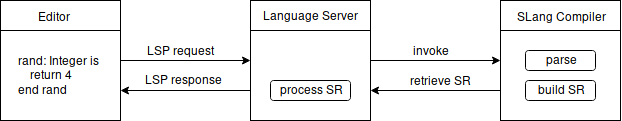
\includegraphics[width=1.0\textwidth]{figs/compiler_integration.png}
    \caption{Workflow with Language Server and integrated compiler}
\end{figure}

\section{Language Server Extensible Architecture}
\label{sec:met:arch}
The main idea of this research is to bring architecture of Language Servers to the next level,
make it modular and extensible, thus allowing third parties to throw in additional functionality for the SLang tooling
with no need to hack into the Language Server code.

Therefore, the architecture of the SLang Language Server is divided into two aggregate components:
\begin{itemize}
    \item The Core
    \item Module System 
\end{itemize}
Where the Language Server Core is a framework through which the Modules do operate.

\begin{figure}[H]
    \centering
    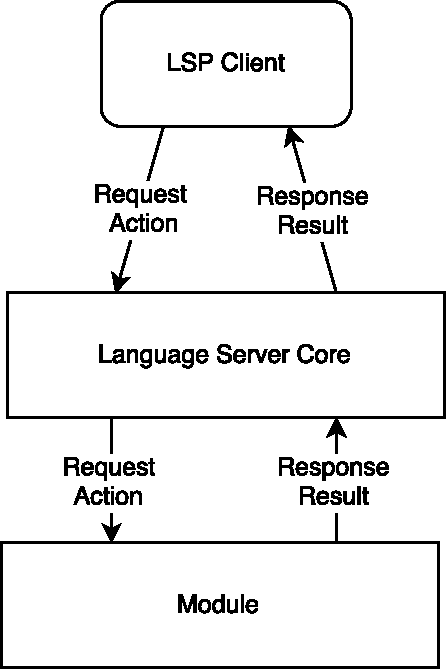
\includegraphics[width=.3\textwidth]{figs/highlevel_architecture.pdf}
    \caption{Language Server High-level Architecture}
\end{figure}

\subsection{Language Server Core}
\label{sec:met:arch:core}
Language Server Core is a basement level of the Language Server on which Language Server Modules will operate.
Responsibilities of LS Core include:
\begin{itemize}
    \item LS Client connection maintenance
    \item Module registry maintenance
    \item Routing of incoming requests and data control flow between modules
\end{itemize}

Each of these responsibilities we shall describe in detail.

\subsubsection{Client connection maintenance}
\label{sec:met:arch:core:connection_maintenance}
According to Language Server Protocol\cite{Sourcegraph}, client controls the lifetime of a server, 
i.e starts it and shuts the server down on demand. After startup, client connects to the server
using one of transports. Since the transport level is not constrained by the LSP, specific transport 
can vary in different implementations.

Language Server Core should support several transports and be able to operate on them to accept requests 
and respond to the client. The list of widely used transports we will implement is
\begin{itemize}
    \item stdin/stdout
    \item tcp
    \item udp
\end{itemize}
Implementing that list will supply the most of LSP clients with an option of how to work with the SLang Language Server.  

\subsubsection{Module Registry}
\label{sec:met:arch:core:module_registry}

To be a foundation for an extensible modular architecture Language Server Core needs to have a subsystem 
for modules registering, maintenance and their inter-operation organization.

\begin{figure}[H]
    \centering
    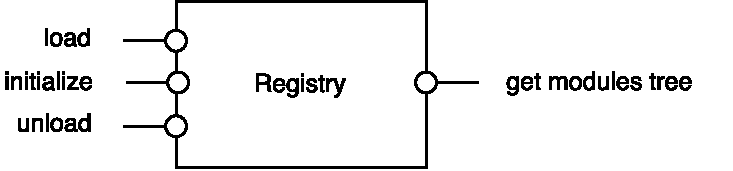
\includegraphics[width=.7\textwidth]{figs/registry.pdf}
    \caption{Module Registry API}
\end{figure}

\newpage
The registry should register and give module status, as well as information how to launch and connect
internal (core) and external modules. On startup, registry should initialize it's state using a predefined directory
containing configuration files. Afterwards, it should maintain an API to load and unload additional modules via LSP.
Consequently, we need to extend the LSP with additional commands for the modules registry:

\begin{itemize}
    \item registryCtl/load
    \item registryCtl/unload
    \item registryCtl/status
\end{itemize}

\subsubsection{Routing and data flow control}
\label{sec:met:arch:core:dispatcher}

After startup, connection setup, module registering and initialization, 
Language Server accepts the first request from the client. 
This request gets validated by Language Server Core, then, after looking up the Module Registry, the request 
gets handed over to the beginning of processing pipeline, responsible for handling this type of requests.

Basically the dispatcher part is a glue, that connects all Language Server components together and 
maintains the data flow ``edges" for the modules graph, enabling module inter-operation by the
rules loaded into the Registry and that are discussed further in the section \ref{sec:met:arch:ms}.

There is a simpler alternative approach to organize module inter-operation: let the modules send data 
to each other and organize pipeline as they want. Although peer-to-peer schema here will save a lot of bandwidth, 
it will also inevitably lead to the dependency hell, 
as such approach would require having every module knowing each other and to connect to each other. 
Thus, here we face the classic client/server trade-off: we can offload a ``server" (LS Core) only
if we will complicate a ``client" (modules). 
Since the client side is to be developed by third parties, the simpler it is -- the better: 
server, controlling all data flow will leave the module developer only with the business logic implementation tasks. 

\subsection{Module System}
\label{sec:met:arch:ms}

Language Server is a great idea to enable IDE-like functionality for
the comparably simple text editors, but currently they are mostly designed as 
a monolithic software, while their service functions are naturally extensible: 
e.g it's common for the static analyzer to have modules for different diagnostics.

Similarly, one of Language Server functions is to provide editor with diagnostics: here we can 
have at least two modules hierarchy -- the compiler diagnostics and the diagnostics provided by an external static analysis tool.
We can even go further and implement a static analyzer as a base static analysis module and a bunch of atomic diagnostic modules derived 
from this base module. 
The same logic is applicable to every Language Server service to some extent.

Separation of the monolithic core from the actual functionality implemented through modules
will significantly lower the Language Server internal bonding, and will make
module implementation relying on a stable API possible, therefore allowing the core and modules
development to be performed simultaneously with no mutual API breakages.

Therefore another value of an extensible architecture that we can derive is 
Language Server easy adoption for any specific corporate needs. 
As implementing some additional functionality would be as easy as developing a plug-in using 
the Language Server Modules API, corporate users can extend the Language Server 
due to their specific requirements, i.e add custom diagnostics, enforce code style, 
or even hook-up the proprietary static analysis or code generation tools.

\begin{figure}[H]
    \centering
    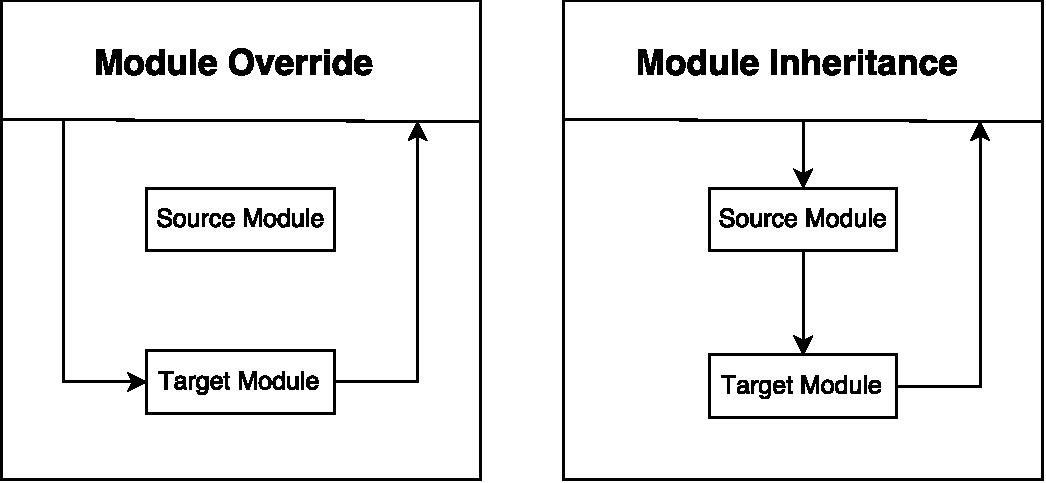
\includegraphics[width=.7\textwidth]{figs/module_hierarchy.pdf}
    \caption{Module Hierarchy}
\end{figure}

One of the ways to develop such architecture was already introduced above: the hierarchy of modules, 
expressed with the basic Object-Oriented Programming terms. In the module hierarchy
modules can either override other modules or extend them in a way of post-processing the
results of base module computation. So the modules would form a classic tree, deriving from a base module,
and intercepting the data flow.

\begin{figure}[H]
    \centering
    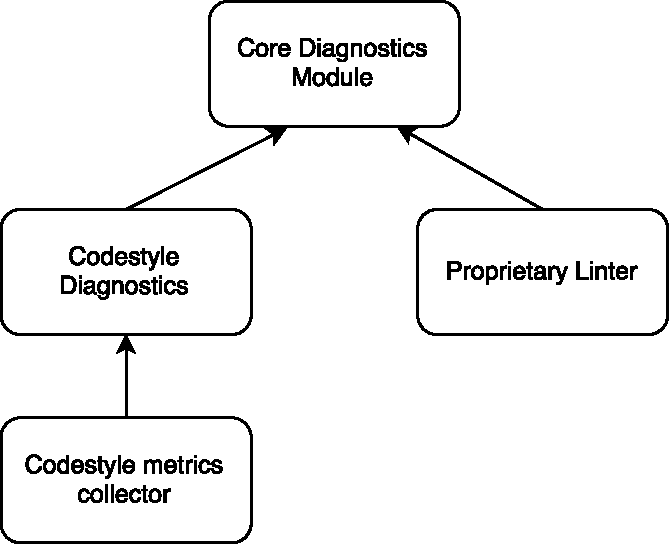
\includegraphics[width=.5\textwidth]{figs/module_tree.pdf}
    \caption{Modules Tree}
\end{figure}

Having this as a basement of the modular system architecture, we can derive a 
neat easy-to-use API to build the modules.

We have a notion of the base and derived modules. Taking as an example the modern Object-Oriented languages` 
type systems, we can build a hierarchy with the base modules, distributed with the Language Server, and responsible for
one particular LS Protocol method. These modules will mainly provide the basic run-time for all the derived modules: 
\begin{itemize}
    \item set up data types: the input information, analysis context, and the results.  
    \item perform the construction of the context (if applicable).
    \item intercept analysis results of the derived module and send it to the client through LSP.
\end{itemize}

As one could have figured, it is not really a usual O-O inheritance: core modules don't let 
the derived ones to override their logic as they work with the Language Server Client and therefore
are forced to live within the same process with the Language Server due to resources sharing. 

Hereby, we have two types of modules:
\begin{itemize}
    \item Core Modules: embedded into the LS process, exposing the run-time for external modules, can not be overridden.
    \item External Modules: plugable things, derived from the core modules, can be overridden.
\end{itemize}

\begin{figure}[H]
    \centering
    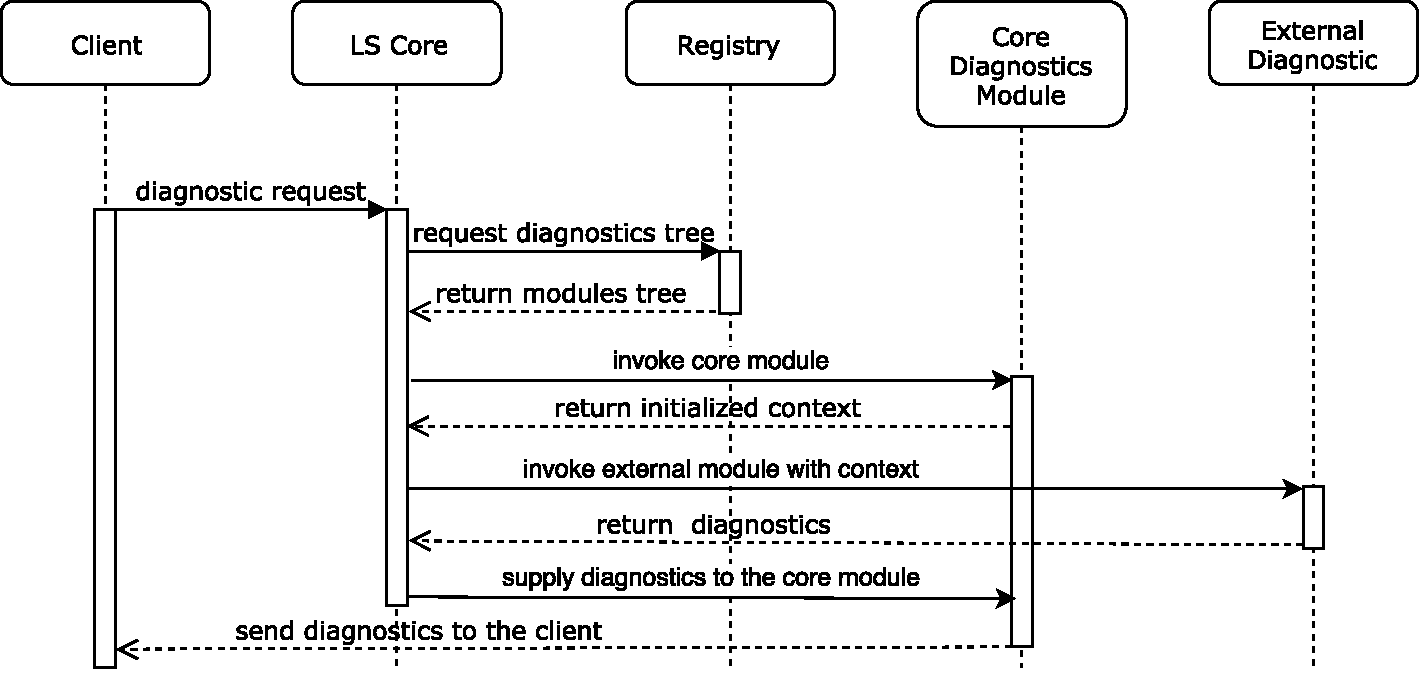
\includegraphics[width=1.0\textwidth]{figs/modules_sd.pdf}
    \caption{Modules invocation sequence diagram}
\end{figure}

Summing up, now we have a way to integrate the compiler into the Language Server, powerful extensible architecture,
that allows to throw in additional functionality for the Language Server, 
and modules hierarchy to start designing the core modules for the Language Server Protocol methods, as well as
the external ones to perform actual analysis and supply Language Server Clients with the code insights.

\section{Development Plan}
To implement a complex system it is vital to split the work into chunks and introduce
the iterative development plan, that would cover a small self-contained part of work on each iteration,
in such way that the result of each iteration could be presented as a working product.

Also, each iteration should include unit and integration testing to form a good test coverage
at the end of the development and to simplify project evolution through use of regression testing.

\subsection{A Dummy Language Server}
Firstly the very basic functionality will be implemented: 
\begin{itemize}
    \item accepting the connection
    \item handling a diagnostic request with a hardcoded response
\end{itemize}

\begin{figure}[H]
    \centering
    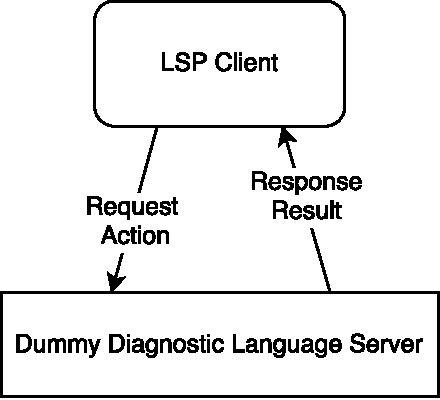
\includegraphics[width=.3\textwidth]{figs/ls_iteration_1.pdf}
    \caption{Iteration 1}
\end{figure}

\newpage
\subsection{SR-driven Language Server}
The next step would be to integrate a compiler and it's Semantic Representation
to feature semantic highlights for the SLang Language Server.
\begin{figure}[H]
    \centering
    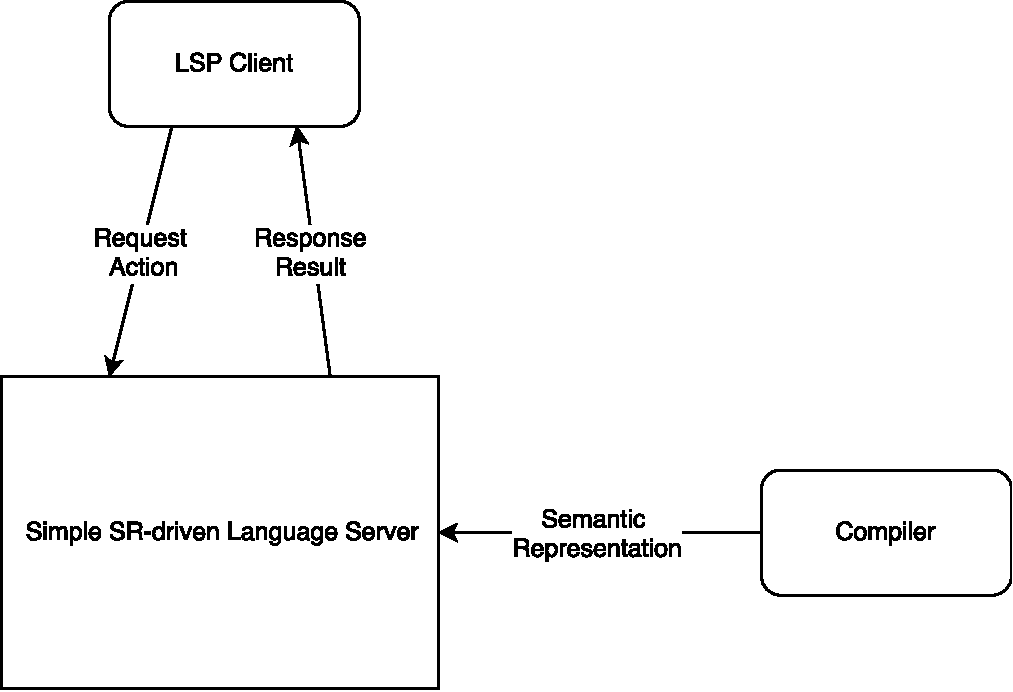
\includegraphics[width=.6\textwidth]{figs/ls_iteration_2.pdf}
    \caption{Iteration 2}
\end{figure}

\subsection{Basic Modular Language Server}
After all the groundwork with the protocol and compiler inter-operation, 
modular architecture implementation may be started: without foreign process extensions for now,
including only built-in modules, that operate in the same address space with the Language Server,
and the simple registry for them, to mock the basement for the future extensible LS.

\begin{figure}[H]
    \centering
    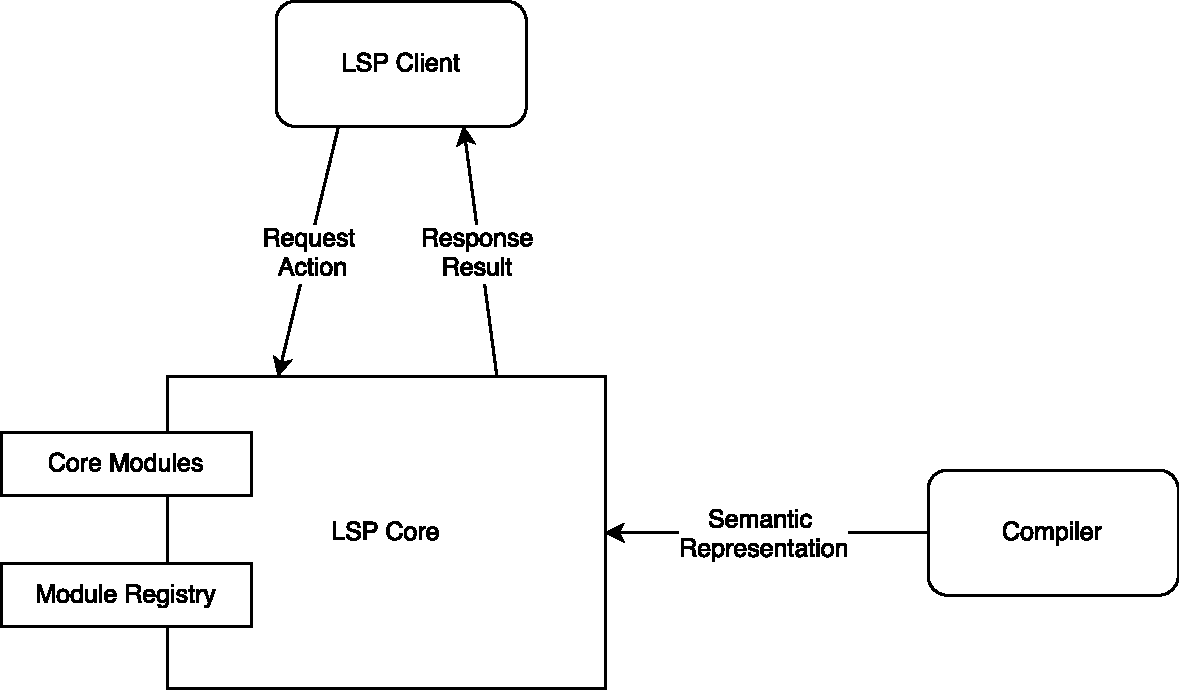
\includegraphics[width=.6\textwidth]{figs/ls_iteration_3.pdf}
    \caption{Iteration 3}
\end{figure}

\subsection{Extensible Language Server}
Finally, the last step will be to extend the registry so it would handle configuration files
and load external modules and to extend the inner protocol and API to work with modules, that are operating
in external processes.
Thus completing the extensible Language Server implementation for SLang.

\begin{figure}[H]
    \centering
    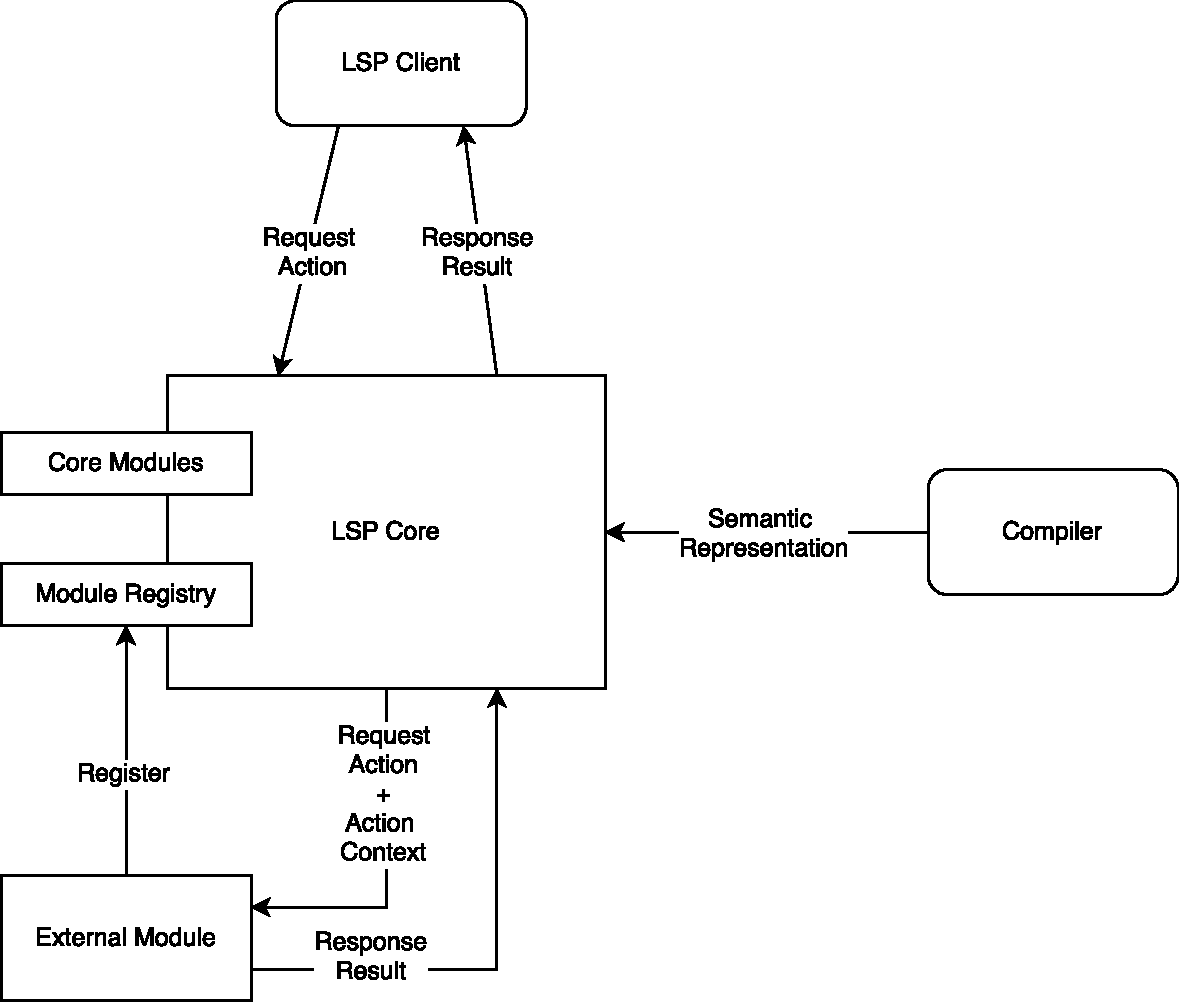
\includegraphics[width=.6\textwidth]{figs/ls_iteration_4.pdf}
    \caption{Iteration 3}
\end{figure}



 


% \section{Basic Language Server Modules}
% \label{sec:met:mods}
% \subsection{Code Semantic Based Highlights Module}
% \label{sec:met:mods:highlights}
% Architecture and methods of IR analysis for highlights

% Mapping from semantic entities to LSP highlighting staff

% \subsection{Autocomplete Module}
% \label{sec:met:mods:autocomplete}
% Description if autocomplete algorithms and data structures choice